% Tikz File 'mytikz.tex'
\documentclass{standalone}
\usepackage{amsmath,xparse}
\DeclareMathOperator{\vsd}{VSD}
\DeclareMathOperator{\asd}{ASD}
\DeclareMathOperator{\ea}{EA}
\DeclareMathOperator{\bb}{BB}
\DeclareMathOperator{\voc}{VC}
\usepackage{tikz}

\pgfdeclarelayer{bg} 
\pgfdeclarelayer{background}
\pgfdeclarelayer{foreground}
\pgfsetlayers{background,main,foreground}
\tikzstyle{sensor}=[draw, text width=2em, 
    text centered, minimum height=2.5em]
 \tikzstyle{v} =[circle, thick, minimum size=0.8cm, draw=black]

\begin{document}
   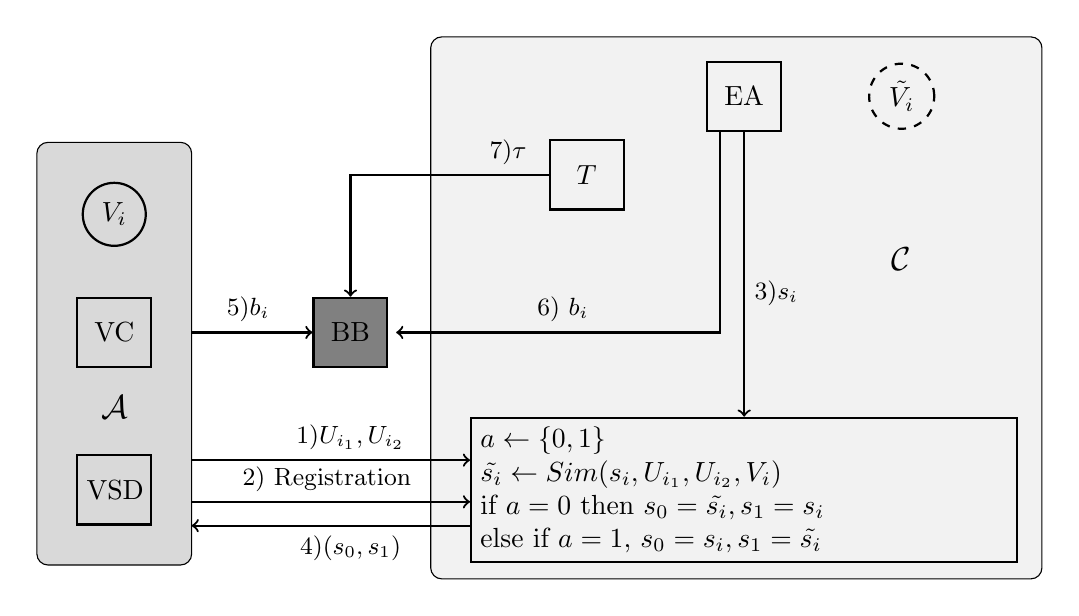
\begin{tikzpicture}[thick]
  \node[draw,rectangle]  at (6, 10) (ea)[sensor] {$\ea$};
  \node [draw,circle] at (-2,8.5) (v)[v]{$V_i$};
   \node [dashed, draw,circle] at (8,10) (vfake)[v]{$\tilde{V_i}$};
  
  \node[draw,rectangle]  at (-2, 5) (vsd)[sensor] {$\vsd$};
    \node[draw,rectangle]  at (4, 9) (tr)[sensor] {$T$};
      \node[draw,rectangle]  at (-2, 7) (vc)[sensor] {$\voc$};
  \node[draw,rectangle,text width=6.7cm]  at (6, 5) (c) {$a \leftarrow \{0,1\} $  \\ $\tilde{s_i} \leftarrow Sim(s_i,U_{i_1},U_{i_2},V_i)$ \\ if $a = 0$ then  $s_0 = \tilde{s_i}, s_1 = s_i$\\ else if $a=1$, $s_0=s_i, s_1 = \tilde{s_i}$  };
   \node[draw,rectangle, fill =  gray]  at (1, 7) (bb)[sensor] { BB};
   \path (vc.south) +(-0,-0.5) node (a) {\large{$\mathcal{A}$}};
   \draw[transform canvas={xshift=-2ex},->,shorten >=0.4cm] (ea) node[font=\small, above,xshift=-2cm,yshift = -3 cm]  {6) $b_i$}  |- (bb);
   
   \draw[transform canvas={yshift=-1ex},->,shorten <=0.5cm]  (vsd) node[font=\small, above,xshift=2.7cm] {$2)$ Registration} -- (c);
   \draw[transform canvas={yshift=-3ex},->,shorten >=0.5cm] (c) node[font=\small, below,xshift=-5cm]  {$4) (s_0, s_1)$}  -- (vsd);
    \draw[transform canvas={yshift=2.5ex},<-,shorten >=0.5cm] (c) node[font=\small, above,xshift=-5cm]  {$1) U_{i_1}, U_{i_2}$}  -- (vsd);
    \draw[->,shorten <=0.5cm] (vc) node[font=\small, above,xshift=1.7cm] {$5) b_i$} -- (bb);
    
      \draw[->] (tr) node[font=\small, above,xshift=-1cm] {$7)  \tau $} -| (bb);
    
   \draw[<-] (c) node[font=\small, right,yshift=2.5cm] {$3) s_i$} -- (ea);
    
       \begin{pgfonlayer}{background}
        \path (vc.west |- v.north)+(-0.5,0.5) node (e) {};
        \path (vsd.south -| vsd.east)+(+0.5,-0.5) node (d) {};
        \path[rounded corners, draw=black, fill = gray!30]
            (e) rectangle (d);
    \end{pgfonlayer}
    
  
       \begin{pgfonlayer}{background}
        \path (c.west |- ea.north)+(-0.5,0.3) node (a) {};
        \path (c.south -| c.east)+(+0.3,-0.2) node (b) {};
        \path[rounded corners, draw=black, fill = gray!10]
            (a) rectangle (b);
    \end{pgfonlayer}
    \path (c.north) +(+2,2) node (RE) {\large{$\mathcal{C}$}};
  \end{tikzpicture}
\end{document}